he general equation of a circle is
\begin{align}
   \vec{x}^T\vec{x}+2\vec{u}^T\vec{x}+f=0\label{eq:solutions/1/4/1} \\
   \text{If $r$ is radius,  }f=\vec{u}^T\vec{u}-r^2\\
   \text{center }\vec{c}=-\vec{u}
\end{align}

Given centre is \myvec{2\\2}
\begin{align}
    \implies \vec{c}=\myvec{2\\2}\\
    \implies \vec{u}=\myvec{-2\\-2}
\end{align}
Equation \eqref{eq:solutions/1/4/1} becomes
\begin{align}
  \vec{x}^T\vec{x}+\myvec{-4&-4}\vec{x}+f=0\label{eq:solutions/1/4/2}
\end{align}
This passes through point \myvec{4\\5}\\
Substituting $\vec{x}=\myvec{4\\5}$ in \eqref{eq:solutions/1/4/2}
\begin{align}
\myvec{4&5}\myvec{4\\5}+\myvec{-4&-4}\myvec{4\\5}+f=0\\
\implies f=-5
\end{align}
Also, radius can be determined as follows
\begin{align}
  f=\vec{u}^T\vec{u}-r^2 \\
  \implies -5=\myvec{-2&-2}\myvec{-2\\-2}-r^2\\
  \implies -5=8-r^2\\
  \implies r=\sqrt{13}
\end{align}
The equation of required circle is 
\begin{align}
  \vec{x}^T\vec{x}+\myvec{-4&-4}\vec{x}-5=0
\end{align}
See Fig. \ref{eq:solutions/1/4/Fig}

\begin{figure}[!ht]
\centering
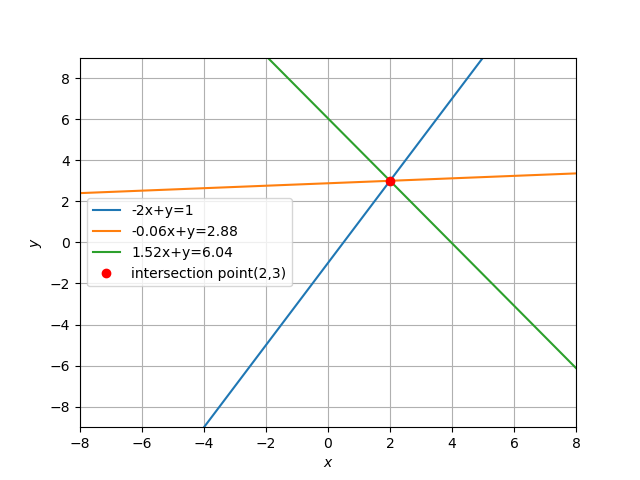
\includegraphics[width=\columnwidth]{./solutions/1/4/plot.png}
\caption{plot showing the circle}
\label{eq:solutions/1/4/Fig}
\end{figure}
